% !BIB TS-program =
\documentclass{svproc}
\usepackage{url}
\usepackage{hyperref}
\usepackage{graphicx}
\usepackage{amsmath}
\usepackage{algorithm}
\usepackage{tabularx}
\usepackage[noend]{algpseudocode}
\usepackage{todonotes}
\def\UrlFont{\rmfamily}
\tolerance=1
\emergencystretch=\maxdimen
\hyphenpenalty=10000
\hbadness=10000
\hypersetup{
  colorlinks=true,
  linkcolor=blue,
  filecolor=magenta,
  urlcolor=cyan,
  citecolor=black,
}

\begin{document}
\mainmatter
\title{Analysis of different AI Strategies for Solving Picross Puzzles}
\subtitle{CS7IS2 Project (2020/2021)}
\author{Andrej Liadov, Edvinas Teiserskis, Min Wu, Edmond Cheng, Adam McQuade}
\authorrunning{A. Liadov, E. Teiserskis, M. Wu, E. Cheng, A. McQuade}
\institute{
  \email{liadova@tcd.ie}, \email{teiserse@tcd.ie}, \email{wumi@tcd.ie}, \email{chenge@tcd.ie}, \email{amcquade@tcd.ie}}

\maketitle              % typeset the title of the contribution


\begin{abstract}
Research in Artificial Intelligence has always had a very strong relationship with games and game-playing. Picross (a.k.a nonograms) are logic puzzles with simple rules and challenging solutions, and in this case our research provides a survey that analyses and compares different AI algorithms - uniform cost search, Q-learning, constraint satisfaction problems (CSPs) and genetic algorithms (GA) applied to solve picross puzzles. Through the process of implementation and evaluation we analyse there algorithms and find out their common aspects, differences, connections between methods, drawbacks and open problems.
\keywords{artificial intelligence, uniform cost search, Q-learning, constraint satisfaction problems, genetic algorithms}
\end{abstract}


\section{Introduction}
Artificial intelligence (AI), in our scope, is the application of computing to solve non-trivial problems and analyse complex, real-world, situations.
AI has been extensively researched and applied to many situations at this point in time. However, the basis of testing many AI approaches remains in the application of AI to well defined games, such as chess, and logic puzzles such as Sudoku or, in our case, Picross.

Picross, also known as Nonograms, is a logic puzzle in which the player uses provided rules to mark (or omit from marking) cells in a grid.
The rules are given as a ordered list of numbers, each referring to a contiguous sequence of filled cells in the grid.
The puzzles come in two formats, monochrome and multicoloured.
Cell sequences must be separated, either by a space in same-colour sequences, or a break by a sequence of a differing colour.
Typically, the rules are given as lists of numbers at the sides of the grid (see Figure 1). As these puzzles (typically) have only one solution, the best method to solve them is determined by the speed of the solution.
We decided on looking at picross puzzles due to their relative novelty, and we were also attracted by the goal of solving a puzzle being to produce an image - a quality that Sudoku cannot compete with.

\begin{figure}[h]
  \centering
  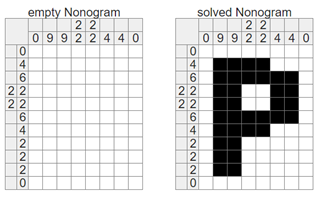
\includegraphics[width=0.6\textwidth]{picross1.png}
  \caption{An example of a picross puzzle, with the start state on the left and completed puzzle on the right. The numbered hints describe how many contiguous blocks of cells are filled. Black cells mark filled cells and blank cells mark unfilled cells. Example from \texttt{https://en.wikipedia.org/wiki/Nonogram}, sourced 2021-04-28.}
\end{figure}

Our goal is to analyse the solving of picross puzzles, and determine which is the best among the 4 approaches we are examining. These types of results can be used for picross design feedback, content generation, or difficulty estimation.
One potential use is to act as an automated difficulty grading system to be used by picross puzzle designers. Depending on the approach and the time taken to solve the puzzle by a given algorithm, a puzzle curation system can sort puzzles in terms of their difficulty.
For example, there are dozens of documented strategies for picross\cite{picross1}, and puzzle designers construct puzzles and rank their difficulty based on which of these strategies are used\cite{picross2}.

This paper presents a comparison of 4 different AI algorithms - uniform cost search, Q-learning, CSP and GA - that we  have decided to apply to solving picross puzzles.
The paper also evaluates these algorithms based on their execution time, memory usage and other metrics.
Through the process of implementation and evaluation we show the pros and cons of each algorithm, and we also examine their common aspects and differences, connections between methods, drawbacks and open problems.
Our recording of presentation link of this research is xxx. \todo[inline]{get recording link - maybe put in a different location in the report?}


\section{Related Work}
Picross, like other logic puzzles such as Sudoku, has a solution that can be reached by the applications of rules of the puzzle, with no strict ordering.
In Sudoku, the squares are filled with one number each while in Picross each cell is either filled in with a colour or left blank.
Prior work has examined the solutions of these puzzles, but most existing solvers are programs written from scratch for the explicit purpose of solving picross puzzles\cite{5.1.1,5.1.2,5.1.3,5.1.7}.
Browne provides a deductive search algorithm that is intended to mimic the constraints and method of human solvers\cite{Browne}.
The complexity of picross can be estimated by calculating the number of steps that can be solved one row/column at a time according to Batenburg and Kosters\cite{Batenburg and Kosters}.

Heuristic search is a technique that uses a heuristic value for optimizing the search.
Heuristic solving involves steps applied in order to determine the value of cells in a single row or column\cite{Salcedo}, in order to decide upon which cells can be assigned based on that value\cite{CHYU}.
An example of applying heuristic steps to fill the cells is Teal’s Nonogram Solver\cite{Teal}.
The input for this solver is a string containing the row and column definitions.
The solver runs through all rows and columns one by one, while applying heuristic steps in order to fill cells.
However, the solver leaves several cells undetermined, which can afterwards be filled by applying logical derivations from the puzzle's state.
These are cells that need input from the previous cells in a run, usually at the end of a row or column.
A-star is an example of a heuristic algorithm that is commonly used in pathfinding and graph traversal, which is the method of finding a traversable path in a graph\cite{astar}.

The Backtracking Heuristic (BH) methodology is a combination of a heuristic approach, which applies a mathematical programming model, and a backtrack search algorithm in order to determine the best heuristics and an optimal ordering between them\cite{BH}.

Backtracking Search for Constraint Satisfaction Problems (CSP): Backtracking is a variant of depth-first search.
The difference lies in an extra step backtracking applies.
Each time the algorithm traverses a node (state in our case), the state of the puzzle is checked.
If a constraint is broken, then the algorithm will backtrack to the puzzle's previous state and explore the next branch, rather than continuing down the branch that will not yield a solution.

Reinforcement Learning for CSP: According to Mehta et al.\cite{Qlearning}, the constraints of a logic puzzle, such as Sudoku, could be modelled as an image, and then have deep Q-Learning applied to it in order to solve the logic puzzle.
The agent is trained with no rules of the game, with only the reward corresponding to each state's action.
Mehta et al. contribute to how to determine the reward structure, state representation, and formulation of the deep neural network when applied to the types of logic puzzles we are examining in our own work.

Genetic algorithms have found much use in puzzle-based problem solving.
According to Mantere and Kolijonen\cite{geneticAlgo}, genetic algorithms are well suited for multi-objective optimisation problems, such as sudoku puzzles.
Search algorithms are commonly deployed in games in order to find an optimal solution to a problem with many path options.
A problem encountered by search algorithms is the high time and space complexities required when the search domain becomes exceedingly large.
Genetic algorithms are a way of mitigating this downside of search algorithms with respect to solution searching, and have been demonstrated as effective in solving other constraint based puzzles such as sudoku.

\section{Problem Definition and Algorithm}
We looked at four algorithms in total - search (specifically, Uniform Cost Search), Q-Learning, Constraint Satisfaction and Genetic Algorithms.
We decided on search as an example of an unsuitable approach, q-learning because it provides an informed, albeit somewhat random, backtracking mechanic, constraint satisfaction because of the natural mapping between the puzzle to the approach, and Genetic Algorithms, due to the dissimilarity of the approach from the other ones we were attempting.

\subsection{Uniform Cost Search}
We have implemented an uniform cost search solution to solve picross puzzles - while this is an established search algorithm, this requires our problem to be represented as a searchable graph.

We did this by modelling the puzzle as a graph - The start state is an empty puzzle, and the next states are potential moves of filling in a square as a particular colour, out of all unfilled squares (our only factor of filtering is if a row/column combination allows for a colour).
The cost function we have implemented is looking at the row/column of the square in question, and calculating:

$$ (1 - row_{proportion}) * (1 - column_{propotion}) $$

where $row/column_{proportion}$ is the number of squares of that colour in that row/column divided by the height/width of the puzzle.
As such, in the intersection of a full row/column pair, the action cost is zero, of a nearly full pair close to zero and for a sparse pair approaching one.
This gives us a cost function which makes cheaper locations that will be more likely to contain a square of that colour.

While the original plan was to add onto this a heuristic in order to implement a-star search, we could not come up with a sensible way to derive a heuristic from the state of the puzzle.
We would either produce a calculation that would most likely not correspond to a useful way to estimate the "completeness" of a puzzle, or we would effectively be encoding another method like constraint programming within the heuristic itself (making the surrounding search implementation redundant).

Due to the nature of the puzzle, using search is expected to be the worst performing method, and is mainly created as an example.
Since the puzzle can have an inordinate number of states, and there is a massive expansion of state transitions at each state, using a search approach immediately hits major speed and memory limits.

For example, taking a monochrome 5x5 puzzle, we have $2^{25}$ total possible states, and most states have a numerous amount of state transitions - 25 from the initial state, 24 from \textit{each} state following those, and so on.
As such, the frontier of the search grows at a very rapid pace - this both makes each state take additional computing time, and quickly fills up the physical limits of available memory on most computers.

Some reduction occurs from the fact that the cost and result of two paths leading to the same state are regardless of order, allowing us to collapse in duplicate entries.
However, this does not nearly reduce the load of the approach to a state where is it comparable to other methods that actively check against the puzzle's rules and full current state in a sensible manner.

\subsection{Q-Learning}
First the state space and the actions space had to be defined for the problem in order to create a Q-learning agent.

The state of a given puzzle was defined as the the rows that were filled in by the Q-leaning agent. If there were different permutation chosen for a given row of a given puzzle, the state of the puzzle would be different.

The action space for a given puzzle would be defined by getting the permutations of the row that are left to be filled in. Choosing a row to fill would be considered an action that would consequently move the agent to a different state. If an action is chosen for a row it is not possible to reverse that action. The row would be filled if an action was taken and as a result, there would not be any actions available for that row.

The state space contains two exit states. The first method is to fill in all the rows and to not have any more actions to take. If there are no more actions to take, the algorithm checks whether the solution to the puzzle is correct. If the answer to the puzzle is correct, the reward returned is 1000. If the completed puzzle is incorrect, the reward returned is -100.

Q-learning with a q-table is meant to choose actions in such a way that the reward is maximised. The state space contains very few solutions. In most of the puzzles tested there was a unique correct solution, in some cases there might have been several solutions. Usually the correct solution space is sparse while the incorrect solution space is quite vast. The contrast between correct solution space and incorrect solution space was reflected in the calculation of reward. Taking an action that did not complete the puzzle should always result in a reward of +1. If the an action taken results in a correct solution, a reward returned was +1000 and if the solution was incorrect, a reward of -100 was returned.

The approach to exploration was a soft-max approach. The exploration rate would be high very high to begin with because nothing is known about the reward, action and state space. A high exploration rate encourages the agent to choose random actions. A random number is generated between 0 and 1 and if epsilon is larger than the random number, the agent picks a random action. If not, it picks the action with the highest q-value. Epsilon has a pre-defined decay rate. By the time the episode number reaches 100, the agent will be a hard-max solver, meaning the agent only picks the best q-value at a given state.

The number of episodes will determine how many times the problem will be completed and the q-table will be updated a proportional amount since the q-table is updated after every action. The pseudo-code for an episode is given below.

\begin{algorithm}
	\caption{Q-Learning Algorithm}\label{euclid}
	\begin{algorithmic}[1]
		\For {$\textit{episode} \text{ in } \textit{num\_episodes}$}
		\State $\textit{agent.puzzle} = \textit{read\_puzzle()}$
		\For {$\textit{step} \text{ in } \textit{max\_steps}$}
		\If {$agent.is\_explore()$}
		\State $\textit{action = agent.get\_random\_action()}$
		\Else
		\State $\textit{action = agent.get\_action()}$
		\EndIf
		\State $\textit{new\_state, reward, complete = agent.step(action)}$
		\State $\textit{agent.update\_qtable(action, new\_state, reward)}$
		\State $agent.puzzle = new\_state.puzzle$
		\If{$complete$}
		\State $\textit{break}$
		\EndIf
		\EndFor
		\EndFor
	\end{algorithmic}
\end{algorithm}

Updating the q-table is done the Bellman equation. This process is combines the old q-value with a learning rate, the reward, the discount rate and the max q-value in the future state. The equation is given below. Alpha is the learning rate and it determines how much influence the new q-value will have on the old one. The higher the learning rate, the more influence the future q-value will have on the new q-value.

\begin{equation}
	NewQ(s, a) = (1 - \alpha)Q(s,a) + \alpha[R(s,a) + \gamma maxQ'(s', a') - Q(s,a)]
\end{equation}

\subsection{Constraint Programming}
The basis of the constraint programming algorithm applied was backtracking, with constraint propagation. Depth first search was used as the backend to apply backtracking. The algorithm starts off with an empty puzzle. All permutations of the first row are generated and filtered. The filtering process here refers to  constraint propagation. Constraint propagation is applied as follows:

\begin{enumerate}
    \item Generate all permutation of row
    \item For each row, check if the column constraint is broken. A column constraint is broken when that column does not contain that colour.
    \item Return list of all feasible rows
\end{enumerate}

The returned list of rows is used to set the states of the backtracking algorithm. Every time a row is set into the nonogram puzzle, the state of the nonogram is checked. Every column in the puzzle is checked. If the number of occurrences of any given colour is greater than the what the constraints dictate, then that row is removed. Figure \ref{fig:Backtrack} below displays this process. This checking is done every time a new row is added.

\begin{figure}[h]
    \centering
    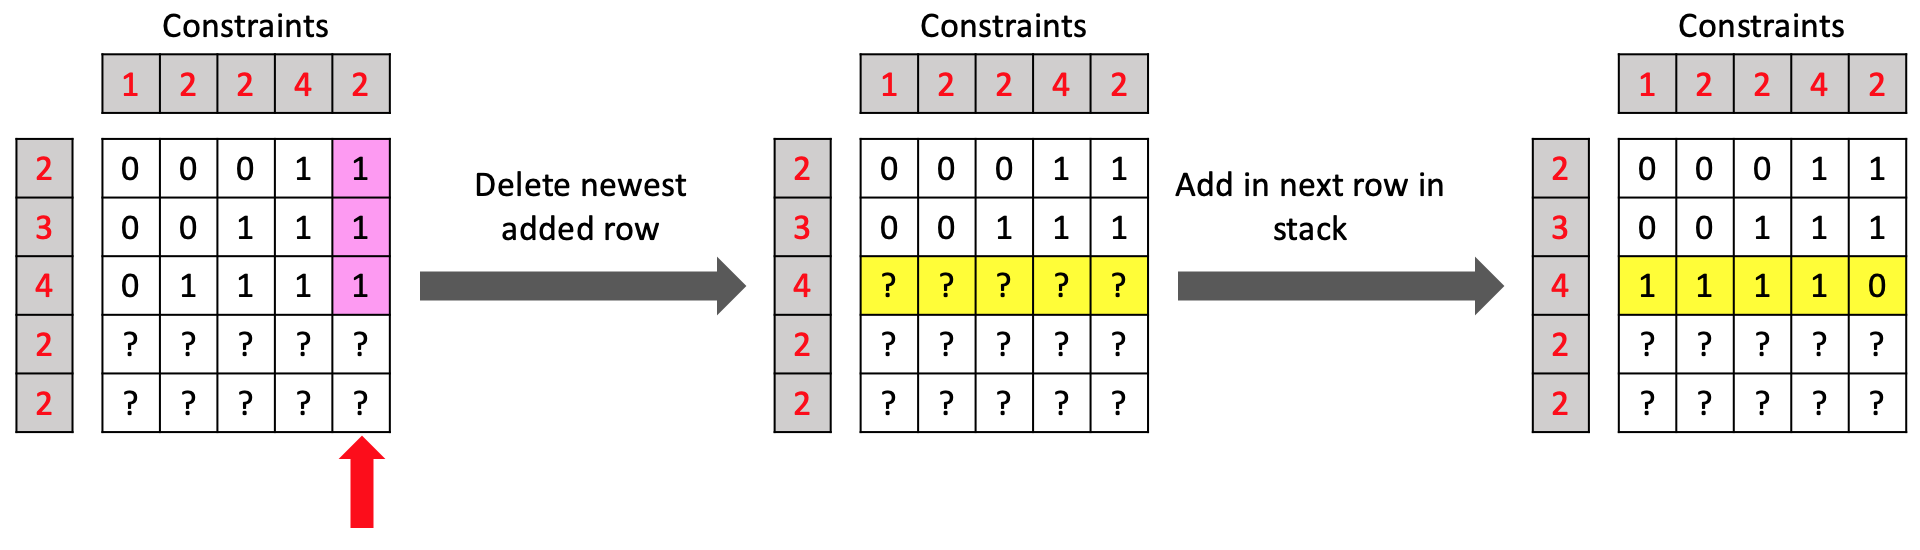
\includegraphics[scale=0.36]{Backtracking.png}
    \caption{Backtracking}
    \label{fig:Backtrack}
\end{figure}

The overall algorithm is shown below.

\begin{algorithm}
    \caption{CSP Algorithm}\label{euclid}
    \begin{algorithmic}[2]
        \State $\textit{stack} = \text{LIFO\_stack}$
        \State $\textit{all\_rows} = \text{generate\_all\_rows[row\_index]}$
        \State $\textit{viable\_rows} = \text{filter\_rows(all\_rows)}$
        \While {$\textit{stack } \text{!= } \textit{empty}$}
        \State $\textit{row} = \text{stack.pop}$
        \State $\text{puzzle.insert\_row(row)}$
        \State $\textit{check} = \textit{puzzle.check\_constraints}$
        \If {$check == False$}
        \State $\text{puzzle.delete\_row(row)} \to \text{continue}$
        \EndIf
        \While {$\textit{index} < \textit{puzzle.height}$}
        \State $\textit{stack.push(generate\_all\_rows(index)}$
        \EndWhile
        \EndWhile
    \end{algorithmic}
\end{algorithm}

\subsection{Genetic Algorithms}
The approach taken in this project follows the typical genetic algorithm design implementation. The programme reads the rules file which determines the constraints for each nonogram puzzle.
\begin{enumerate}
\item Selection:
the parents for the next generation are selected based on a metric known as fitness. In this implementation, fitness is a measure of how many of the constraints are left unsatisfied by a parent solution. The agents are sorted by those with the lowest number of unsatisfied constraints and these are more likely to be parents.

\item Crossover:
is the process of combining the characteristics of two parents to form a child. Using a probability function, a random split of each of two parents characteristics is taken and recombined into a new characteristic. This is undertaken for each pair of parents at the end of an iteration to create the new generation.

\item Mutation: this is the process of randomly altering minor details in the characteristics of the new generation of agents. In this case it implies that a random block within the nonogram will be flipped from filled to unfilled.
\end{enumerate}
The programme terminates in either one of two ways. At the end of each iteration of agents, the solution is checked against that reached by the algorithm and terminates if the solution is reached. However, the programme is still liable to make no progression beyond local optima. To mitigate this, the algorithm is terminated and reinitialised with random values after 1000 iterations.

The overall algorithm is shown below.

\begin{algorithm}
	\caption{Pseudo-code for Genetic Algorithm}
	\label{fig:garun}
	\begin{algorithmic}
		\State $population \gets GenerateInitialPopulation(desiredPopulationSize)$
		\State $population \gets assignFitnessToEachMember(population)$
		\While{$run-time < allowedTime$}
		\State $newGeneration \gets selectMembersOfPopForCrossover(population)$
		\State $newGeneration \gets mutatePopulation(newGeneration)$
		\State $population \gets assignFitnessToEachMember(population)$
		\If{$highestFitnessInPopulation(population) >= fitnessRequired$}
		\State \Return $fittestMemeberOfPopulation(population)$
		\EndIf
		\EndWhile
		\State \Return $fittestMemeberOfPopulation(population)$

	\end{algorithmic}
\end{algorithm}

\section{Experimental Results}
	All algorithms were tested using 6 variations of nonograms:
	\begin{itemize}
	    \item 5x5 Monochrome
	    \item WxH Monochrome - where W,H < 10
	    \item 10x10 Monochrome
	    \item 5x5 Multicoloured
	    \item WxH Multicoloured - where W,H < 10
	    \item 10x10 Multicoloured
	\end{itemize}
\noindent All algorithms were allowed a total of 3 minutes to solve the nonogram.
The average solve times under each category are shown in figures \ref{fig:SolveTimes} and \ref{fig:SolveTimesShort}.

One important property to note is that the context of these solve  times matter.
Not all algorithms managed to solve every single nonogram.
Only the backtracking algorithm (hereby referred to as CSP) managed to solve all nonograms.
The specifics are shown in the table below.
\begin{table}[h]
    \centering
    \begin{tabularx}{\textwidth}{|m{0.208\textwidth}||m{0.12\textwidth}|m{0.12\textwidth}|m{0.12\textwidth}|m{0.12\textwidth}|m{0.12\textwidth}|m{0.12\textwidth}|}
        \hline
         CSP & 0 & 0 & 0 & 0 & 0 & 0 \\
         \hline
         Search & 5 & 9 & 10 & 9 & 10 & 10 \\
         \hline
         Q-Learning & 2 & 5 & 10 & 2 & 7 & 10 \\
         \hline
         GA & 2 & 2 & 5 & 10 & 10 & 10 \\
         \hline
    \end{tabularx}
    \caption{Number of Unsolved Nonograms}
    \label{tab:UnsolvedTable}
\end{table}

\begin{figure}[h]
    \centering
    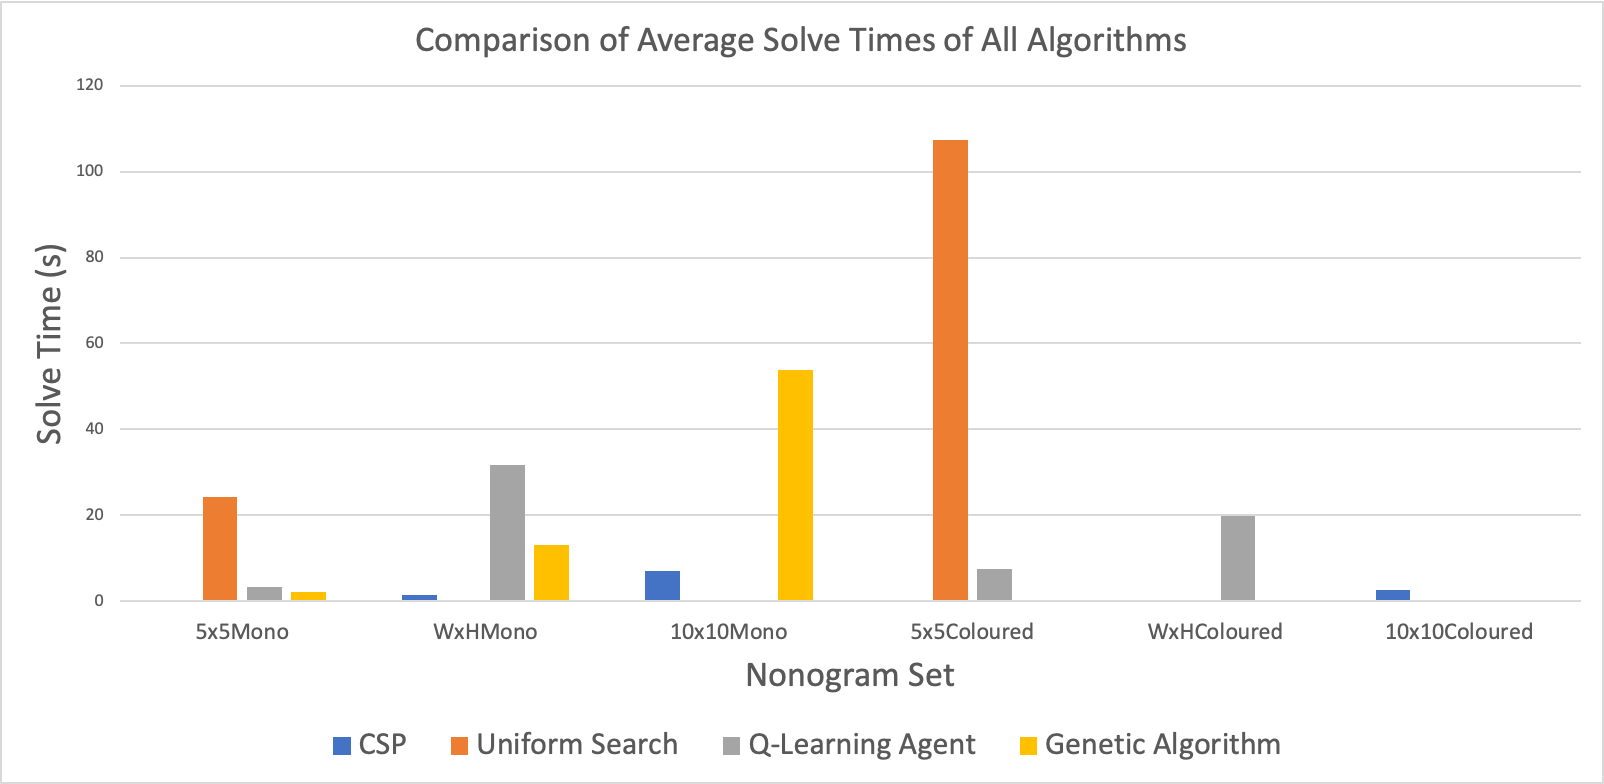
\includegraphics[width=\textwidth]{SolveTimes.png}
    \caption{Average Solve Times of All Algorithms}
    \label{fig:SolveTimes}
\end{figure}

\begin{figure}[h]
    \centering
    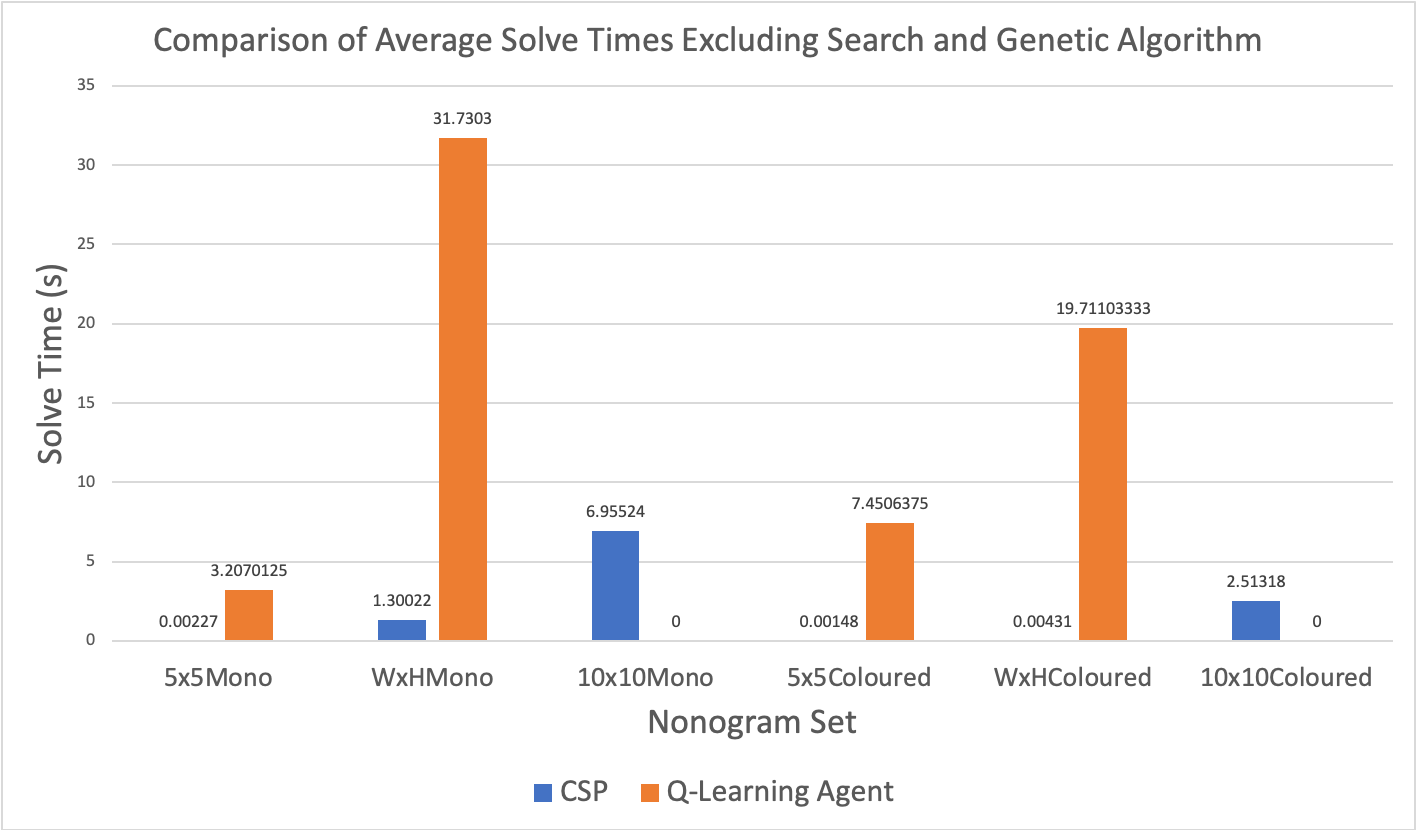
\includegraphics[width=\textwidth]{SolveTimesShort.png}
    \caption{Average Solve Times Excluding Search}
    \label{fig:SolveTimesShort}
\end{figure}
\clearpage

The two criteria the algorithms were judged on were solve time and solve rate. The algorithm that best fit these criteria is the CSP algorithm.
Not only did it solve every single nonogram, it also achieved the lowest average times.
This is contrasted to arguably the worst performing algorithm, which is the uniform cost search.
Search only accomplished a solve rate of roughly 12\% and was the slowest solving algorithm under all categories.
The placements for the genetic algorithm, and the q-learning algorithm are debatable.
They both shared similar solve rates, at 35\% and 30\% respectively.
Their average solve times were comparable, judging from figure \ref{fig:SolveTimes}, but genetic algorithms seemed to scale better with the size of the puzzle.
Q-learning did not scale as well, and fails to solve a single 10x10 nonogram within the 3 minute window.
Genetic algorithm solved 5 of the 10x10 monochromes, and 0 of the 10x10 multicoloured nonograms. The addition of the colour dimension to the genetic algortihm added a level of complexity that could not be solved trivially. For the monochrome tests, the genetic algorithm assumed all nonograms were of the same colour and thus this was not a factor in the analysis.
An argument can be made for either algorithm being superior. Q-learning is more flexible in that it has the capability (somewhat) to solve multicoloured nonograms, whereas genetic algorithm does not. But the solve times using Q-learning increases much quicker than the genetic algorithm solve times. This is especially true in the case of genetic algorithms for which there is a degree of chance to finding a solution quickly or reaching a local optimum and ceasing progression. The mutation aspect of the genetic algorithm is the source of this discrepancy in solve times. If a random mutation leads to a part of the solution being reached quickly, this will lend a huge advantage in completing the remainder of the puzzle. However, the converse is also true; a mutation may hinder the completion of the puzzle such that a parent generation produces a weaker generation of children. The mutation function must balance the likelihood of these two scenarios.

As expected, when the size of the puzzle increased, the solve times also rose correspondingly.
Which leads to results where the algorithms fail to solve the puzzle within the given 3 minute time frame.
While it may be possible that any of the tested algorithms would reach a solution eventually, this process may take too long and take too much memory.
This is the case with the search algorithm.
Search is extremely poor at solving nonograms due to the large state space.
Hence it consumes a lot of memory and time, for very little output.

\section{Conclusions}
In conclusion the most suitable algorithm for picross problems are constraint search problems.
The reason for this is due to the nature of the problem structure. Picross problems requires a solver to mechanically consider many different options and to choose them in a way that will reduce the problem.
This conclusion is exemplified in the results illustrated in figure \ref{fig:SolveTimes}.
Backtracking is powerful for these problems because while it considers the entire state space, it quickly discards options when they fail to conform to the constraints.

In contrast, it is not practical to determine the solution without applying the constraints - meaning a pure action-cost model does not notably improve the solving process. Neither is to judge how far away a particular state is from a solution - therefore creating a heuristic for the problem is incredibly difficult. As such, an informed search approach like our uniform cost search does not introduce problem reduction like the constraint search approach, and as a result the performance is lacking. There was massive memory consumption and time for almost no solved problems.

This reasoning also applies to both Q-learning and genetic algorithm. They fail to scale in performance when the size of the nonogram increases. And eventually, they will fail to solve the puzzle within a limited time frame. Hence if we wanted to scale the nonograms to larger sizes the only realistic algorithm would be backtracking.

Perhaps it could be possible to combine backtracking to q-learning and genetic algorithms. This in turn could reduce the action space for both the genetic and q-learning approaches. As a result, the algorithms might converge on larger problems.


\begin{thebibliography}{6}

\bibitem {Browne}
Cameron Browne. 2013. Deductive search for logic puzzles. In Computational
Intelligence in Games (CIG), 2013 IEEE Conference on. IEEE.

\bibitem {Batenburg and Kosters}
K Joost Batenburg and Walter A Kosters. 2012. On the difficulty of Nonograms.
ICGA Journal 35, 4 (2012), 195–205.

\bibitem {5.1.1}
Jan Wolter's pbnsolve Program
\url{https://webpbn.com/pbnsolve.html}

\bibitem{5.1.2}
Mirek and Petr Olšák's Nonogram Solver
\url{http://www.olsak.net/grid.html#English}

\bibitem{5.1.3}
Steve Simpson's Nonogram Solver
\url{http://www.comp.lancs.ac.uk/~ss/software/nonowimp/}

\bibitem{5.1.7}
Jakub Wilk's Nonogram Solver
\url{http://jwilk.nfshost.com/software/nonogram.html}

\bibitem{Teal}
\url{http://a.teall.info/nonogram}

\bibitem{Salcedo}
S. Salcedo-Sanz, E.G. Ort’iz-Garc’ia et al., Solving Japanese Puzzles with
Heuristics, IEEE Symposium on Computational Intelligence and Games,
2007, 224-231, CIG, 2007.

\bibitem{CHYU}
C.H. Yu, H.L. Lee, L.H. Chen, An efficient algorithm for solving nonograms, Springer Science+Business Media, Springer Verlag, Applied Intelligence 35(1): 18-31, 2011

\bibitem{Peter}
Norvig, Peter. "Solving Every Sudoku Puzzle". Peter Norvig (personal website). Retrieved 24 December 2016.
\url{http://www.norvig.com/sudoku.html}

\bibitem{lecture}
Zelenski, Julie (July 16, 2008). Lecture 11 | Programming Abstractions (Stanford). Stanford Computer Science Department.
\url{https://www.youtube.com/watch?v=p-gpaIGRCQI}

\bibitem{picross1}
Andrew C Stuart. 2007. The Logic of Sudoku. Michael Mepham Publishing.

\bibitem{picross2}
Andrew C Stuart. 2012. Sudoku Creation and Grading. (January 2012).
\url{http://www.sudokuwiki.org/Sudoku Creation and Grading.pdf}
[Online, accessed 8 Mar 2017].

\bibitem{Qlearning}
Mehta, Anav. "Reinforcement Learning For Constraint Satisfaction Game Agents (15-Puzzle, Minesweeper, 2048, and Sudoku)." arXiv preprint arXiv:2102.06019 (2021).

\bibitem{astar}
Solving 8-Puzzle using A* Algorithm
\url{https://blog.goodaudience.com/solving-8-puzzle-using-a-algorithm-7b509c331288}

\bibitem{geneticAlgo}
T. Mantere and J. Koljonen, "Solving, rating and generating Sudoku puzzles with GA," 2007 IEEE Congress on Evolutionary Computation, 2007, pp. 1382-1389, doi: 10.1109/CEC.2007.4424632.
\url{https://doi.org/10.1109/CEC.2007.4424632}

\bibitem{BH}
Jonatã L., Araújo P., Pinheiro P.R. (2011) Applying Backtracking Heuristics for Constrained Two-Dimensional Guillotine Cutting Problems. In: Liu B., Chai C. (eds) Information Computing and Applications. ICICA 2011. Lecture Notes in Computer Science, vol 7030. Springer, Berlin, Heidelberg.

\end{thebibliography}

\end{document}
